\xiaosi

\subsubsection{布线拓扑搜索结果}

经过15代进化搜索（种群16，并行评估），搜索到的最优布线为：中间神经元$n_i = 3$，命令神经元$n_c = 7$，感觉扇出$f_s = 3$，中间扇出$f_i = 5$，命令循环连接$r_c = 0$，运动扇入$f_m = 2$。搜索出的拓扑共15个神经元，较手工设计的25个减少40\%。

\begin{table}[H]
  \centering
  \caption{手工设计与搜索出的NCP拓扑在4个场景上的对比}
  \label{tab:hand_vs_searched}
  \wuhao
  \begin{tabular}{lccccc}
    \hline
    拓扑 & 神经元数 & highway-v0 & merge-v0 & intersection-v0 & roundabout-v0 \\
    \hline
    手工设计 & 25 & $34.94\pm0.98$ & $\mathbf{15.00\pm0.58}$ & $2.82\pm0.56$ & $\mathbf{6.63\pm1.13}$ \\
    搜索发现 & 15 & $33.88\pm1.50$ & $11.12\pm3.74$ & $\mathbf{3.22\pm0.41}$ & $5.47\pm1.45$ \\
    \hline
  \end{tabular}
\end{table}

图\ref{fig:hand_vs_searched}直观展示了两种拓扑在各场景上的奖励和碰撞率对比。搜索出的拓扑在highway-v0（搜索环境）上与手工设计接近（33.88对34.94），但在未参与搜索的merge-v0和roundabout-v0上性能下降。这说明单环境搜索存在过拟合风险，也从侧面证明了布线拓扑确实对NCP的性能有显著影响——不同的拓扑适合不同的场景特征。

\begin{figure}[H]
    \centering
    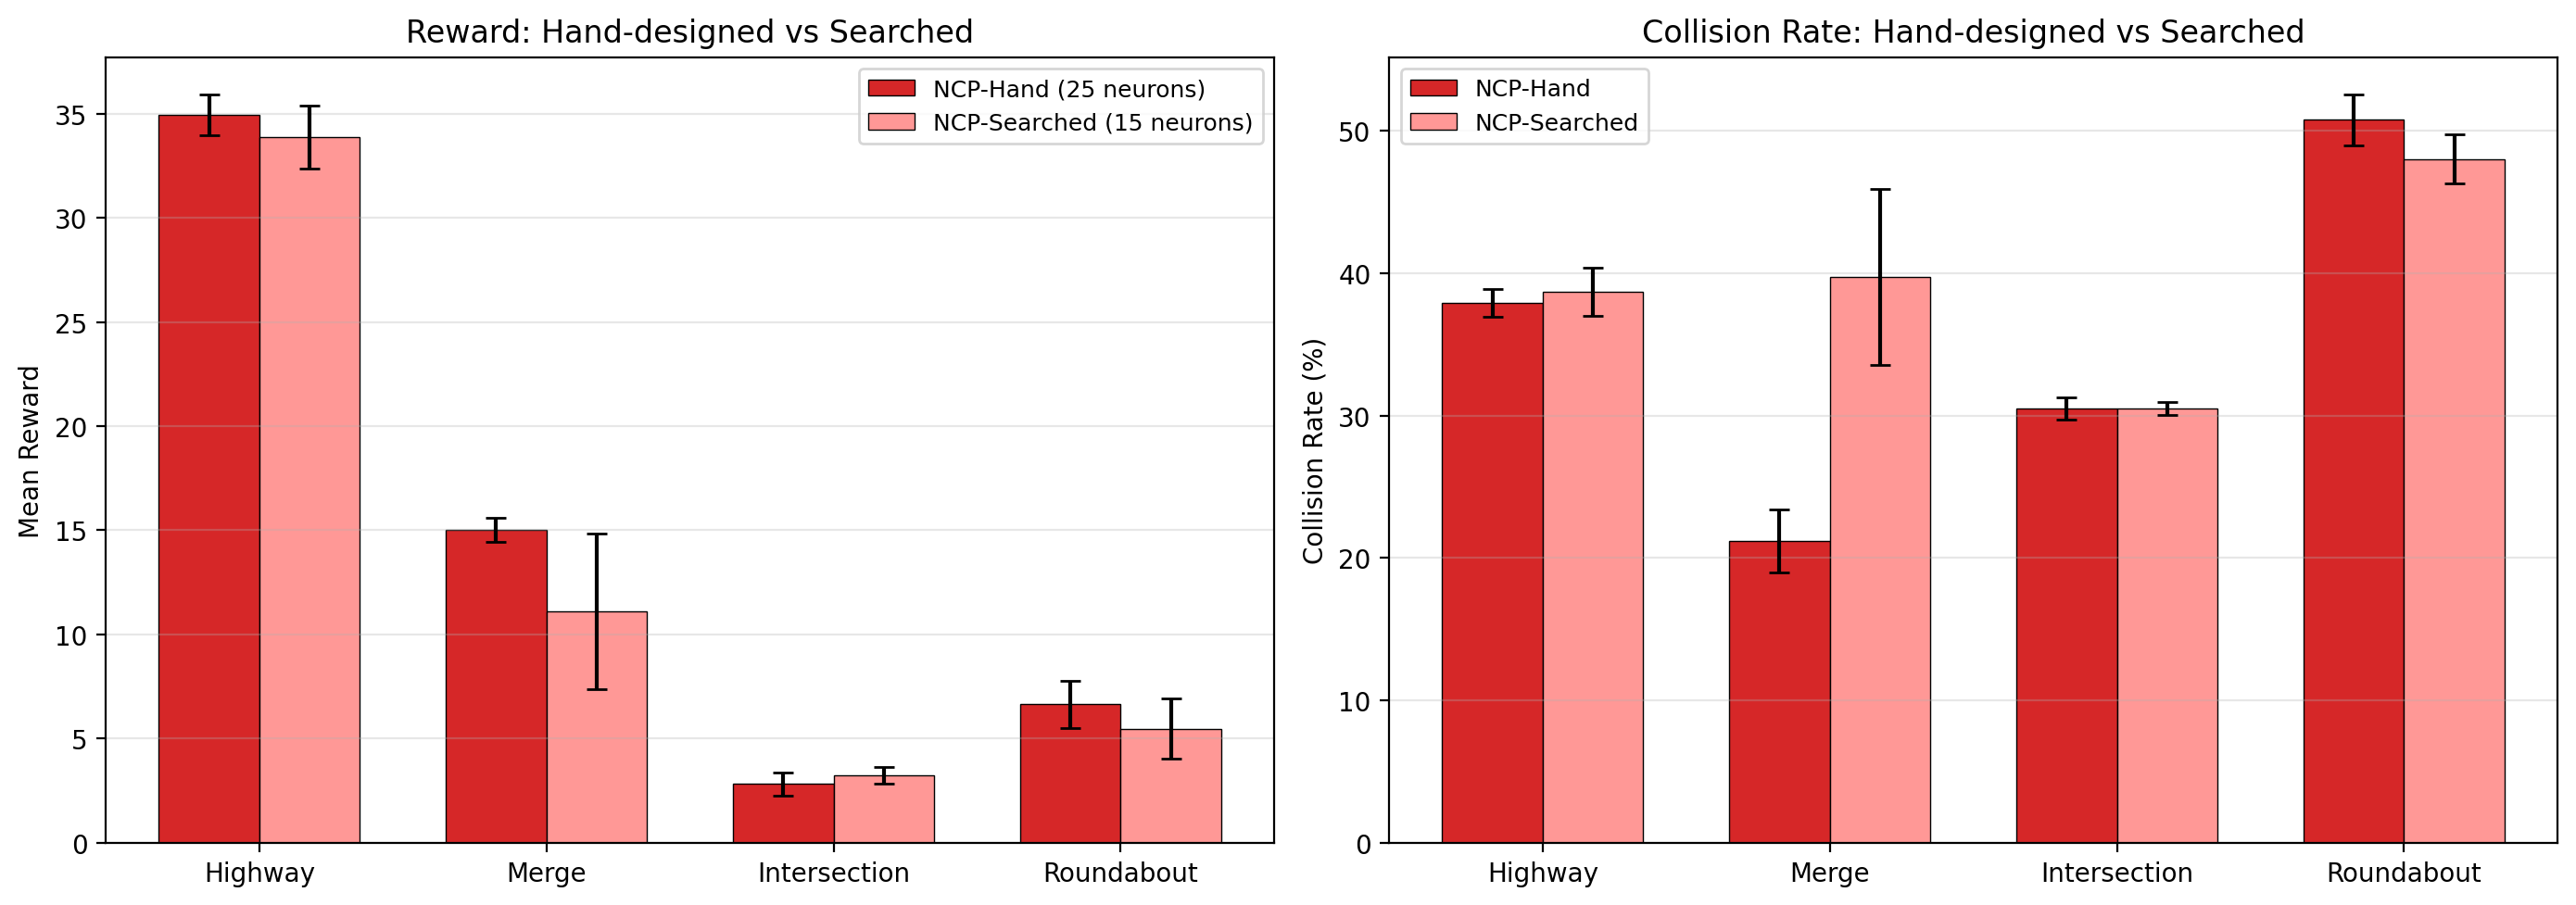
\includegraphics[width=1.0\linewidth]{img/fig_hand_vs_searched.png}
    \caption{手工设计拓扑与搜索拓扑在4个场景上的奖励和碰撞率对比}
    \label{fig:hand_vs_searched}
\end{figure}

搜索收敛曲线（图\ref{fig:search_conv}）显示，最佳适应度在前3代快速上升，之后趋于稳定，说明进化搜索能有效探索布线空间。

\begin{figure}[H]
    \centering
    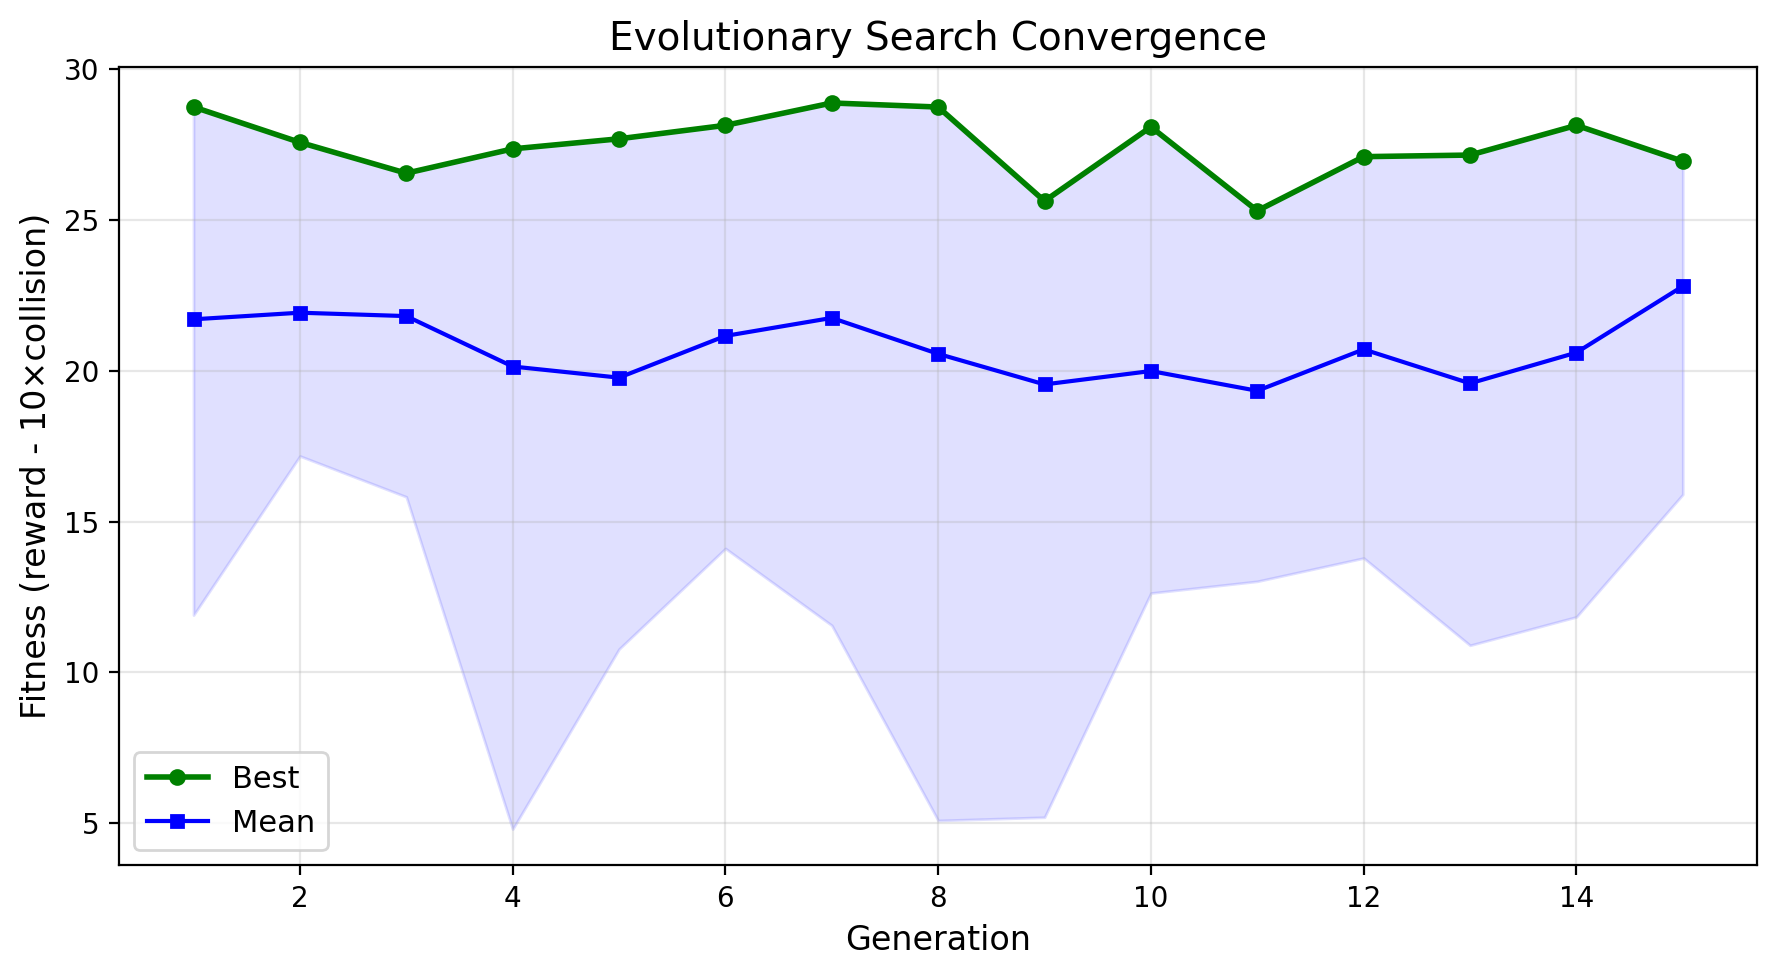
\includegraphics[width=0.8\linewidth]{img/fig_search_convergence.png}
    \caption{进化搜索收敛曲线}
    \label{fig:search_conv}
\end{figure}

\subsubsection{搜索拓扑的结构分析}

图\ref{fig:topo_searched}展示了搜索出的最优拓扑。与第2章图\ref{fig:ncp_wiring_ch2}的手工设计拓扑（25个神经元）相比，搜索拓扑仅有15个神经元，连接更稀疏，且不含命令层内循环连接。

\begin{figure}[H]
    \centering
    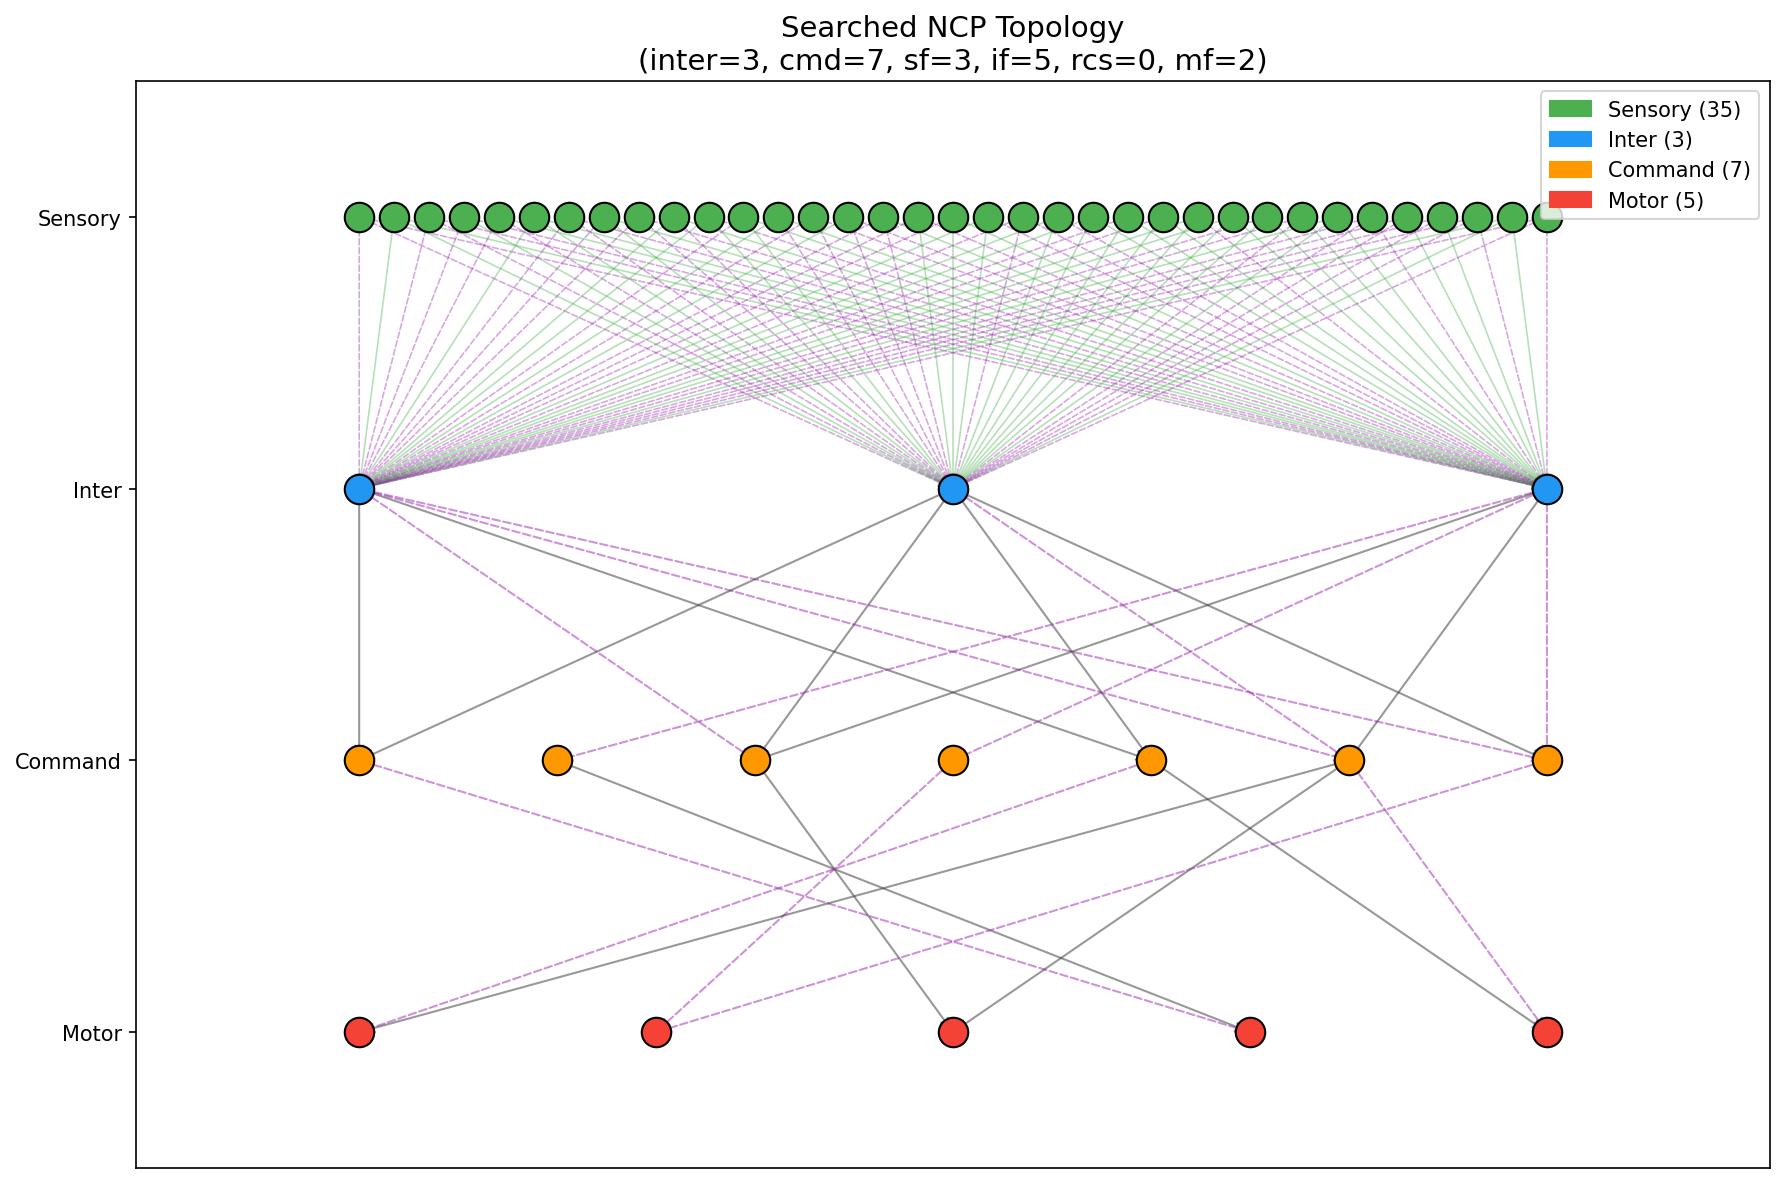
\includegraphics[width=0.75\linewidth]{img/fig_searched_topology.png}
    \caption{进化搜索发现的NCP最优布线拓扑（15个神经元）}
    \label{fig:topo_searched}
\end{figure}

搜索出的拓扑有两个值得关注的特征：（1）$r_c = 0$，即命令层内\textbf{无循环连接}。传统NCP设计认为循环连接对维持短时记忆至关重要，但搜索结果表明，在highway-v0的决策时间尺度上，LTC的ODE动力学本身已提供足够的记忆能力。（2）$n_i = 3$，仅3个中间神经元，表明高速公路场景的信息整合不需要大量中间层冗余。这些发现为NCP的布线设计提供了数据驱动的指导。

\subsubsection{ODE展开数消融实验}

LTC单元中的ODE展开数（\texttt{ode\_unfolds}）控制了每个RNN时间步内Euler积分的迭代次数，是NCP的关键超参数。展开数越多，ODE求解越精确，但计算图也越深。本文在highway-v0上对1、3、6、12四种展开数进行了系统消融，结果如表\ref{tab:ode_ablation}所示。

\begin{table}[H]
  \centering
  \caption{ODE展开数对NCP性能的影响（highway-v0, seed=42, 50000步训练）}
  \label{tab:ode_ablation}
  \wuhao
  \begin{tabular}{cccc}
    \hline
    ODE展开数 & 平均奖励 & 碰撞率 & 相对训练速度 \\
    \hline
    1  & 34.53 & 41.9\% & 1.0× （最快）\\
    \textbf{3}  & \textbf{35.97} & 37.2\% & 0.6× \\
    6（默认）  & 26.61 & 35.1\% & 0.4× \\
    12 & 34.51 & \textbf{34.7\%} & 0.2× （最慢）\\
    \hline
  \end{tabular}
\end{table}

实验得到三个观察：

\textbf{（1）展开数3取得最佳综合性能}。\texttt{ode\_unfolds=3}时reward达到35.97（4个设置中最高），同时碰撞率37.2\%也较低。这表明对于离散决策任务，3步Euler积分已能较好地近似ODE动力学。

\textbf{（2）默认展开数6在本次实验中表现波动较大}。\texttt{ode\_unfolds=6}（NCP论文默认值）在该单一种子实验中reward仅26.61，明显低于其他三个设置。这可能源于该种子下的训练不稳定性，也可能反映了计算图深度对梯度传播的影响——对比基线对比实验（4.2节）中NCP在3个种子上的均值为34.94$\pm$0.98，可见ode=6的实际表现存在较大波动。

\textbf{（3）极端展开数各有取舍}。\texttt{ode\_unfolds=1}训练速度最快（约为默认值的2.5倍），适合资源受限场景；\texttt{ode\_unfolds=12}碰撞率最低（34.7\%），可能更适合对安全性要求极高的场景，但训练速度仅为默认值的一半。

\textbf{局限性说明}：本消融实验仅在单一种子上进行，结论的统计可靠性有限——尤其是\texttt{ode=6}的低reward可能受随机性影响较大。但4个设置之间的总体趋势（reward在26--36之间，方差较大）仍提示：ODE展开数对NCP的训练动力学有显著影响，简单沿用默认值6可能错失更优配置。在工程实践中，建议针对具体任务对此超参数进行调优，3步展开是一个值得尝试的备选。
